\documentclass{article}
\usepackage{bigstrut}
\usepackage{adjustbox}
\usepackage{graphicx}^^M
\graphicspath{ {images/} }
\usepackage[T1]{fontenc}
\usepackage{float}

\usepackage[english]{babel}
\usepackage[utf8]{inputenc}
\usepackage{indentfirst}

\addtolength{\oddsidemargin}{-.875in}
\addtolength{\evensidemargin}{-.875in}
\addtolength{\textwidth}{1.75in}
\addtolength{\textheight}{1in}

\usepackage{hyperref}
\hypersetup{
    colorlinks=true,
    linkcolor=blue,
    filecolor=magenta,      
    urlcolor=cyan,
}

%-----ADDING FIGURES------
%\begin{figure}[h]
%\begin{center}
%\includegraphics[width=\textwidth]{IMAGE_NAME_HERE}
%\caption{CAPTION_HERE}
%\end{center}
%\end{figure}

%-----ADDING TABLES-------
%\begin{table}[h]
%\begin{center}
%\begin{tabular}{c|c|c|c|c}
%& Butterworth & Chebyshev & Linkwitz-Riley & Bessel\\
%\hline
%Passband Accuracy & 10 & 4 & 6 & 9\\
%\hline
%Filter Slope & 7 & 10 & 5 & 6\\
%\hline
%Impulse Response & 5 & 7 & 10 & 3\\
%\hline
%Popularity in Crossover Filters & 3 & 3 & 7 & 3\\
%\hline
%Total & 25 & 24 & 28 & 21\\
%\hline
%Rank & 2 & 3 & 1 & 4\\
%\end{tabular}
%\caption{ADD CAPTION HERE}
%\end{center}
%\end{table}

%-----ADDING IMAGES-----
%\begin{center}
%\includegraphics[width=400px]{Image_NAME_HERE}
%\end{center}


\begin{document}
\title{Sanside Technology}
\begin{titlepage}
    
\includegraphics[width = 150px]{images/SansideLogo.png}
    \hfill
    \hrule
    \vspace{2cm}
    \centering
	{\scshape\LARGE Sanside Technology Mobile Game Design\par}
	\vspace{0.5cm}
	{\scshape Marcin Wisniowski: Product Development Intern \par}
    \vspace{2cm}
    \begin{center}
    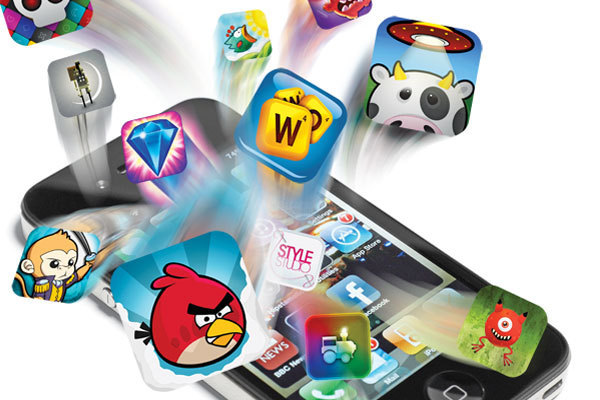
\includegraphics[width = 400px]{images/mobile_game.jpg}
    \end{center}
    \vspace{0.5cm}
    {\scshape A document to help inspire the creation of mobile games}
\end{titlepage}

\pagenumbering{roman}
\section{Abstract}
With WeChat games growing rapidly, there is an important need to find and create game applications at an advanced pace to enter the market during this crutial moment. Due to this, it is important to have a background of games that have been successful in the last few decades and get ideas for games that can also become Internet trends.

\tableofcontents

\newpage
\pagenumbering{arabic}

\section{Review of Popular Lightweight Games on Facebook}
\subsection{Everwing}
Everwing is the most popular Instant Game on Facebook. It can be described as a top-down scroll shooter. The biggest reason it is doing well is because of its social aspect where players can get together and work to defeat a big boss. In the idle-game genre, a lot of games have implemented similar strategies to make players regularly log in to help their teammates. 
\begin{figure}[h]
\centering
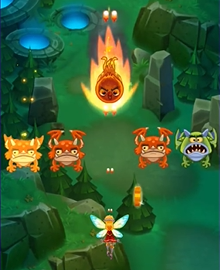
\includegraphics[width=100px]{images/everwing.png}
\caption{Everwing Game}
\end{figure}
\subsection{Sports Games}
Golden Boot and Basketball FRVR are both popular games around the sports gaming category. The mechanics are kept simple by making the user try to score points in both games, but nothing else through swiping the screen. There is always an aspect of increasing the difficulty and giving more points the further you get and the game is very reliant on having a leaderboard to compete with your friends.
\begin{figure}[h]
\centering
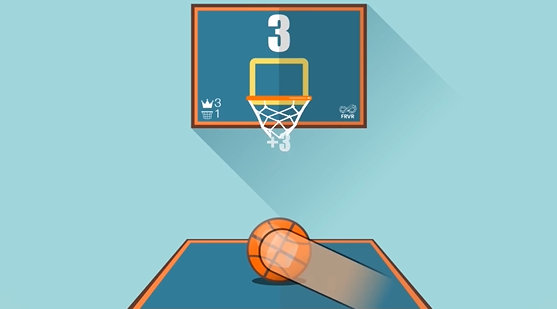
\includegraphics[height = 150px]{images/basketball.png}
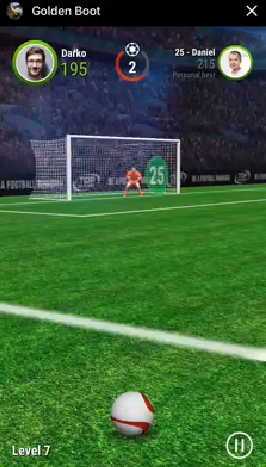
\includegraphics[height = 150px]{images/goldenboot.png}
\caption{Basketball FRVR | Golden Boot}
\end{figure}
\subsection{Board Games}
Other players will look to play board games with other players. Both card games and other board games work well with players taking turns over longer periods of time. Uno, a popular card game in the US was put onto Facebook so that people could play it even when not near each other. Similarly, chess, and Words with Friends (Scrabble) were moved from board games to mobile games.
\begin{figure}[h]
\centering
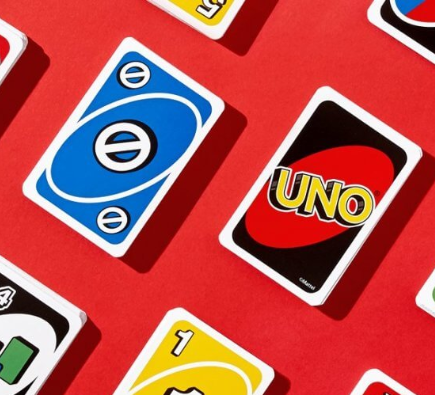
\includegraphics[height = 150px]{images/uno.png}
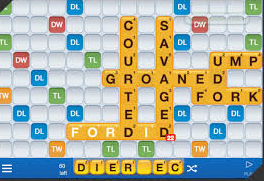
\includegraphics[height = 150px]{images/wordswfriends.png}

\includegraphics[height = 150px]{images/chess.png}
\caption{Uno | Words with Friends | Chess}
\end{figure}
\subsection{Board Games}

\section{Exploration of Social Tendencies in Gaming}
\subsection{Introduction}
Many instant games on Facebook and on mobile devices in general find ways to implement general social rules to games to help bring an audience and their players back to playing the games. The more games you explore on app stores and facebook, the more you can realize what makes a game interesting to play and come back to. Some games may describe these items as increasing the replayability of games and keeping the games interesting. Unless your game has weekly updates to bring new content, a game needs to have at least a few of these or else it will lose its audience.

\subsection{Leaderboards}
Most, if not all, popular mobiles games have leaderboards that are used as a way to track a players progress as well as a way to compare players with each other. Leaderboards come with two main uses:
\begin{enumerate}
\item Global Leaderboards - These look to keep the player engaged by trying to give a reason to keep trying to play the same game over and over. Players try to compete with the rest of the world to try and place as high as possible. Sometimes games have events that take place where the top specific amount of players will receive a reward.
\begin{figure}[h]
\centering
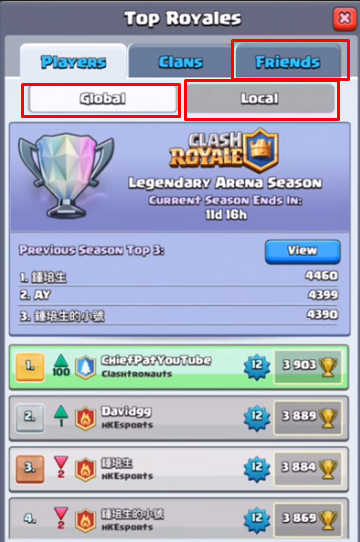
\includegraphics[height = 150px]{images/rankings2.png}
\caption{Global, Local, and Friends Rankings in Clash Royale}
\end{figure}
\item Local Leaderboards - These look to compare players against their friends and really help with creating a competitive nature. Usually, when creating sharing options with leaderboards involved, it is recommended to have local leaderboards where the players listed are interesting to the player.
\end{enumerate}
Another increasingly used mechanic in games is using leaderboards to advance to a harder stage, and therefore splitting the whole games' audience into different tiers of players. Usually these come with ranks that players can boast about in achievements that they can share with friends. 
\begin{figure}[h]
\centering
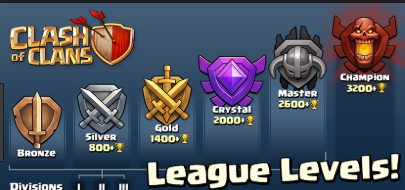
\includegraphics[height = 100px]{images/rankings.png}
\caption{Splitting the community into tiers of leaderboards}
\end{figure}

\section{Further Resources for Game Ideas}
Many simple/instant mobile games have evolved from two main genres of gaming, arcade games and board games. In the 1970s-1990s, when many games were unable to be created with amazing graphics or long stories, a lot of very short but addicting games were released onto arcade machines for people to play on.

\begin{figure}[h]
\centering
 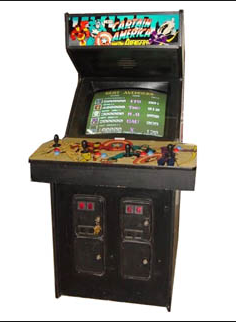
\includegraphics[width = 150px]{images/arcade.png}
\caption{An arcade machine}
\end{figure}
\newpage 

The entire platform looked to create a short game, usually with leaderboards for players to try and reach the highest scores for. Because of this, a lot of instant games can  be traced back to getting their ideas from original arcade games and arcade machines. 

Just by exploring popular arcade games through searching, or through a database, you can get a lot of very good game mechanics to build a new game around. Just remember to always bring your own new twist or art style to the game. 

You can create a game around almost any idea. Just try to find a way to track a person's score while incorporating something that you find interesting. Here are different ways to keep track of leaderboards. Think of what would be the most fun to try and challenge someone else to do:

\begin{enumerate}
\item Score: Collect as many points as you can with different ways of giving them out.
\item Distance: See how far you can go in a level that usually never ends
\item Time: See how fast you can complete something or how long you can stay alive.
\end{enumerate}

\hyperlink{https://en.wikipedia.org/wiki/Arcade_game}{Link to Popular Arcade Games}

\hyperlink{https://archive.org/details/internetarcade}{Play any Arcade Game (Need VPN)}

\hyperlink{https://en.wikipedia.org/wiki/Replay_value}{Replay Value in Video Games}


\end{document}